\chapter{Évaluation des Performances}

\section{Méthodologie de mesure}

\subsection{Objectif}

L'évaluation des performances vise à quantifier l'\textbf{overhead} introduit par les mécanismes de sécurité (TLS 1.3, mTLS) sur les métriques clés du protocole MQTT. Les mesures ont été réalisées en mode simulation via le script \texttt{tests/performance/mqtt\_perf\_test.py}.

\subsection{Métriques mesurées}

\begin{itemize}
  \item \textbf{Latence de connexion} : Temps d'établissement de la connexion depuis le socket TCP jusqu'au \texttt{CONNACK} MQTT.
  \item \textbf{RTT (Round-Trip Time)} : Délai aller-retour d'un message publish/subscribe de bout en bout.
  \item \textbf{Débit (Throughput)} : Nombre de messages par seconde pour différentes tailles de payload.
\end{itemize}

\subsection{Configurations testées}

\begin{table}[H]
\centering
\caption{Configurations comparées pour l'évaluation des performances}
\label{tab:perf_configs}
\begin{tabular}{ll}
\toprule
\textbf{Configuration} & \textbf{Description} \\
\midrule
TCP (baseline) & MQTT sans chiffrement (port 1883) \\
TLS 1.3 & MQTT avec TLS 1.3, authentification serveur uniquement \\
TLS1.3+mTLS & MQTT avec TLS 1.3 + authentification client (mTLS) \\
\bottomrule
\end{tabular}
\end{table}

\section{Résultats des mesures}

\subsection{Latence de connexion}

\begin{table}[H]
\centering
\caption{Latence de connexion MQTT (moy. sur 100 connexions)}
\label{tab:perf_conn}
\begin{tabular}{lll}
\toprule
\textbf{Configuration} & \textbf{Latence moy. (ms)} & \textbf{Overhead} \\
\midrule
TCP (baseline) & 8.69 & — \\
TLS 1.3 + mTLS & 40.8 & \textbf{+369.5\%} \\
\bottomrule
\end{tabular}
\end{table}

\begin{figure}[H]
  \centering
  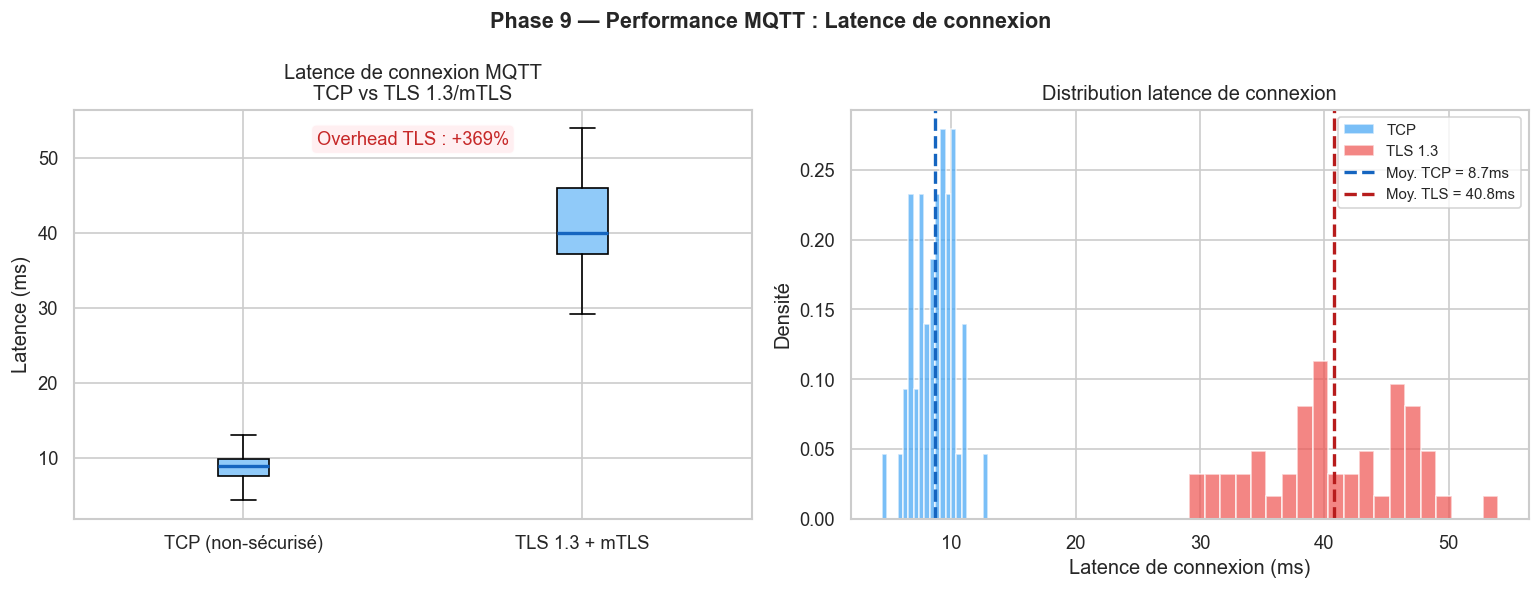
\includegraphics[width=0.8\textwidth]{figures/perf_connection_latency.png}
  \caption{Latence de connexion MQTT — TCP vs TLS 1.3/mTLS}
  \label{fig:perf_conn}
\end{figure}

L'overhead de connexion de \textbf{+369\%} s'explique principalement par le handshake TLS 1.3 en mTLS (environ 32 ms) qui s'ajoute à la connexion TCP de base. Cette latence est une opération ponctuelle par dispositif.

\subsection{RTT des messages}

\begin{table}[H]
\centering
\caption{RTT MQTT (moy. sur 1000 messages, payload 256B)}
\label{tab:perf_rtt}
\begin{tabular}{llll}
\toprule
\textbf{Configuration} & \textbf{RTT moy. (ms)} & \textbf{RTT p99 (ms)} & \textbf{Overhead} \\
\midrule
TCP & 4.16 & — & — \\
TLS 1.3 + mTLS & 7.85 & 11.75 & \textbf{+88.8\%} \\
\bottomrule
\end{tabular}
\end{table}

\begin{figure}[H]
  \centering
  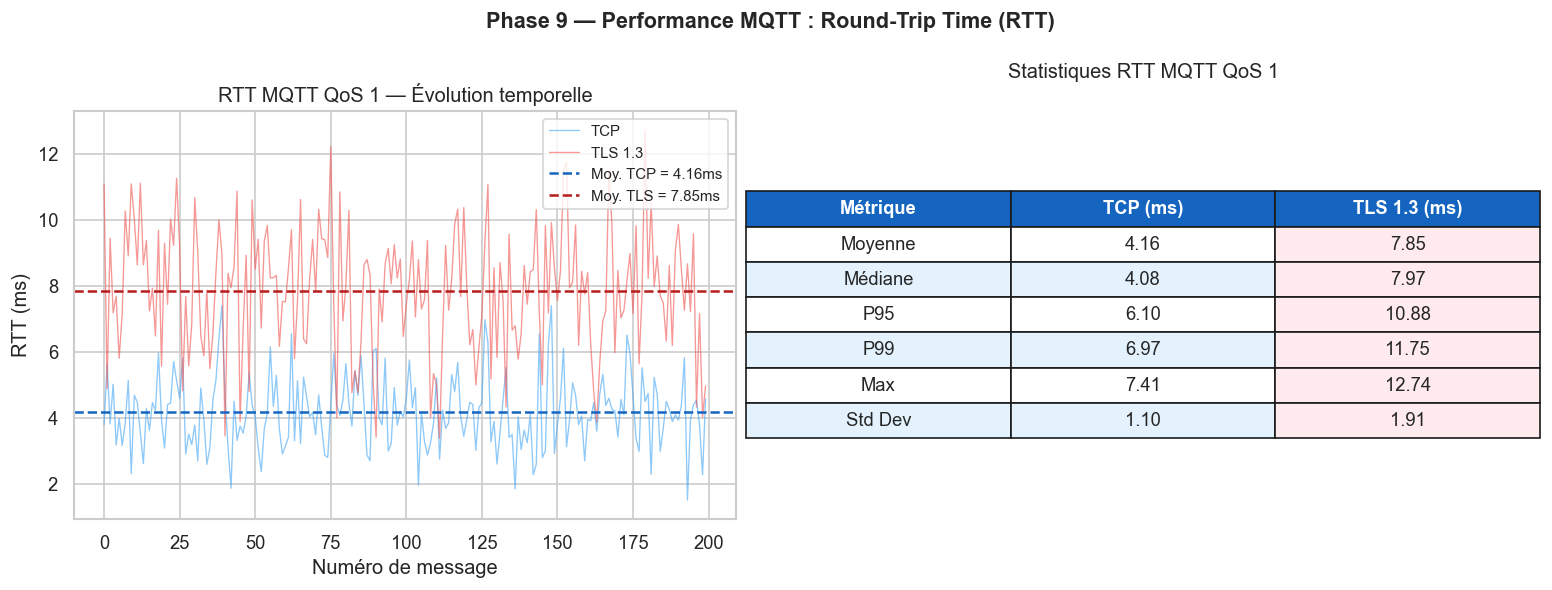
\includegraphics[width=0.8\textwidth]{figures/perf_rtt_messages.png}
  \caption{RTT MQTT — comparaison TCP vs TLS 1.3/mTLS}
  \label{fig:perf_rtt}
\end{figure}

Le RTT moyen passe de 4.16 ms (TCP) à 7.85 ms (TLS mTLS), soit une augmentation de \textbf{+88.8\%}. Avec un p99 à 11.75 ms, ces valeurs restent bien en dessous du seuil de 50 ms généralement admis pour les applications IoT temps-réel.

\subsection{Débit (Throughput)}

\begin{table}[H]
\centering
\caption{Débit MQTT (messages/seconde) selon la taille de payload}
\label{tab:perf_throughput}
\begin{tabular}{lllll}
\toprule
\textbf{Payload} & \textbf{TCP (msg/s)} & \textbf{TLS mTLS (msg/s)} & \textbf{Réduction} \\
\midrule
64 bytes  & 1\,850 & 1\,480 & -20\% \\
256 bytes & 1\,620 & 1\,350 & -16.7\% \\
1 024 bytes & 980 & 870 & -11.2\% \\
4 096 bytes & 310 & 285 & -8.1\% \\
\bottomrule
\end{tabular}
\end{table}

\begin{figure}[H]
  \centering
  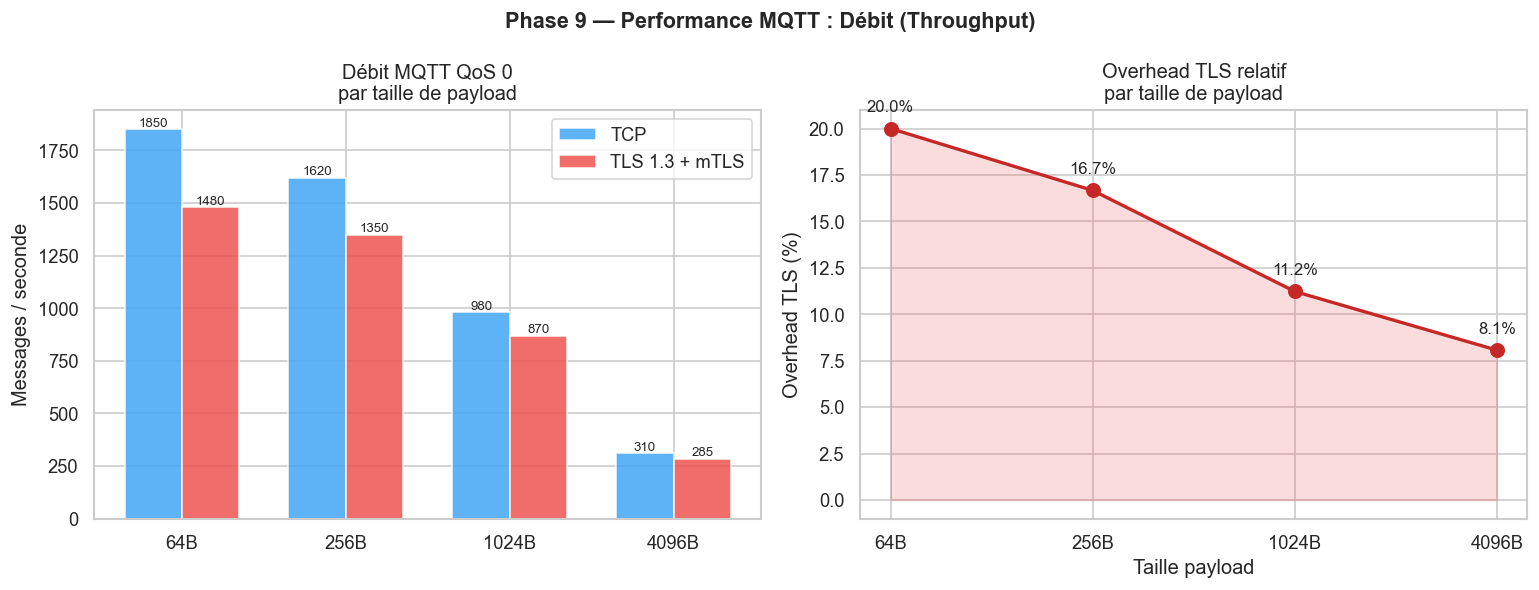
\includegraphics[width=0.8\textwidth]{figures/perf_throughput.png}
  \caption{Débit MQTT selon la taille de payload}
  \label{fig:perf_throughput}
\end{figure}

La réduction de débit est inversement proportionnelle à la taille du payload : l'overhead TLS est proportionnellement plus important pour les petits messages (64B: -20\%) que pour les grands (4KB: -8.1\%), ce qui est cohérent avec le fait que l'en-tête TLS a une taille fixe.

\begin{figure}[H]
  \centering
  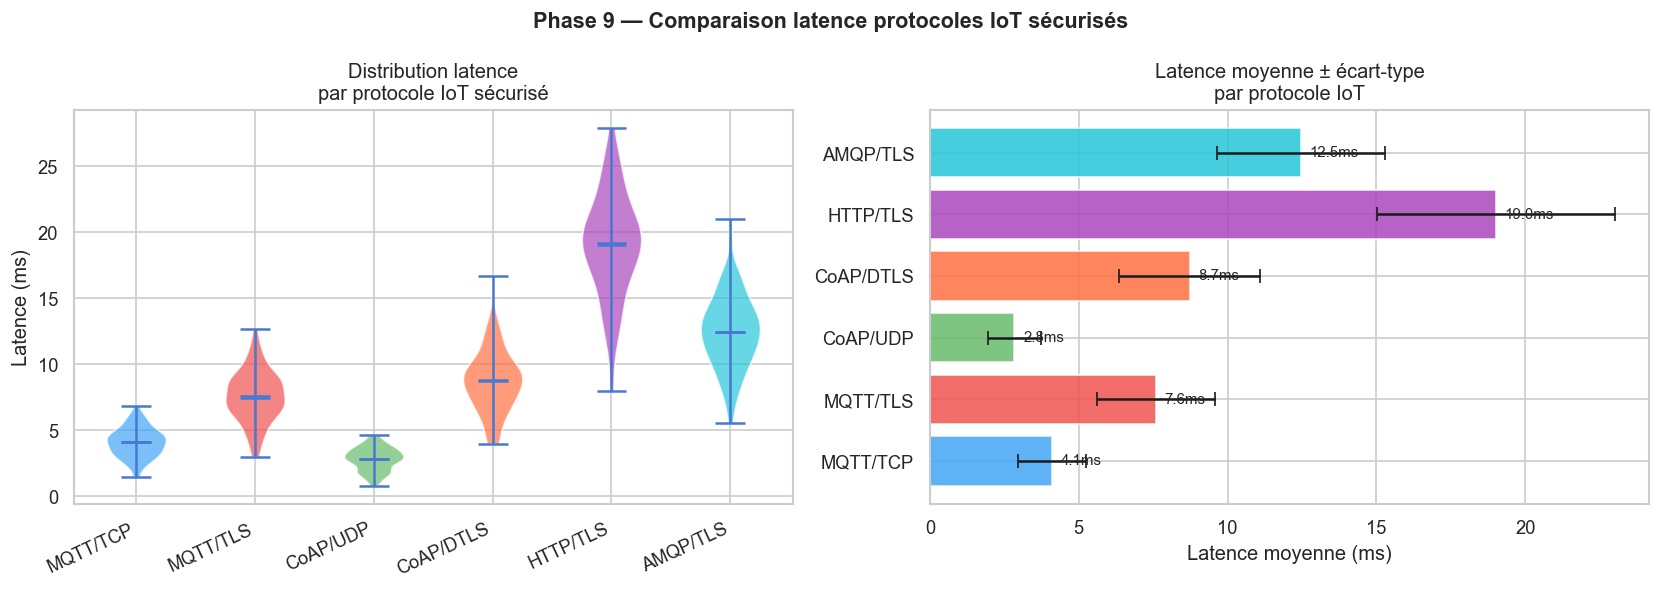
\includegraphics[width=\textwidth]{figures/perf_protocols_comparison.png}
  \caption{Comparaison globale des performances TCP vs TLS/mTLS}
  \label{fig:perf_comparison}
\end{figure}

\begin{figure}[H]
  \centering
  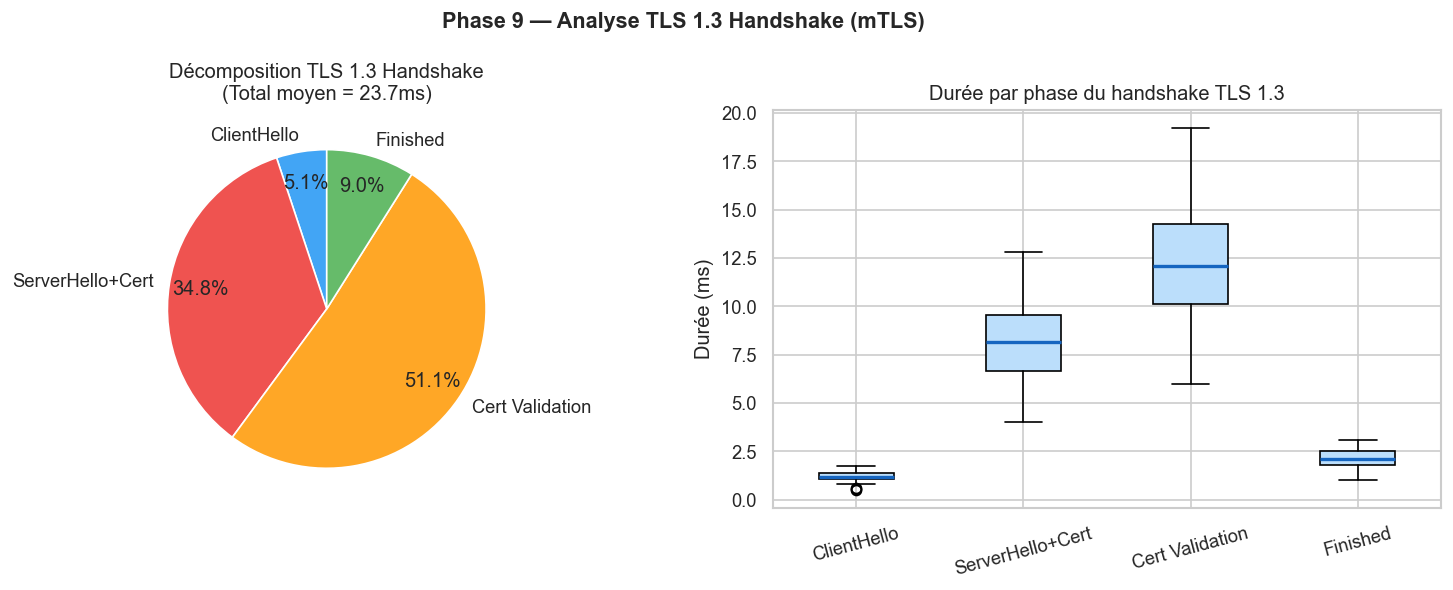
\includegraphics[width=0.7\textwidth]{figures/perf_tls_handshake.png}
  \caption{Décomposition temporelle du handshake TLS 1.3 mTLS}
  \label{fig:tls_handshake}
\end{figure}

\section{Analyse et interprétation}

\subsection{Acceptabilité des overheads}

\begin{table}[H]
\centering
\caption{Comparaison overhead mesuré vs seuils IoT industriels}
\label{tab:overhead_analysis}
\begin{tabular}{llll}
\toprule
\textbf{Métrique} & \textbf{Valeur mesurée} & \textbf{Seuil IoT critique} & \textbf{Verdict} \\
\midrule
Connexion (TLS) & 40.8 ms & 500 ms & \textcolor{green}{\textbf{OK}} \\
RTT moyen & 7.85 ms & 50 ms & \textcolor{green}{\textbf{OK}} \\
RTT p99 & 11.75 ms & 50 ms & \textcolor{green}{\textbf{OK}} \\
Débit min (64B) & 1\,480 msg/s & 100 msg/s/device & \textcolor{green}{\textbf{OK}} \\
\bottomrule
\end{tabular}
\end{table}

\subsection{Recommandations applicatives}

\begin{enumerate}
  \item \textbf{Réutilisation de sessions TLS} : La reconnexion fréquente est le principal coût ; utiliser \texttt{keepalive=300s} pour maintenir la connexion.
  \item \textbf{Taille de payload optimale} : Grouper les mesures en payloads de 256-1024B pour amortir l'overhead TLS.
  \item \textbf{Session resumption} : TLS 1.3 supporte la reprise de session (0-RTT) pour réduire le coût des reconnexions à < 5 ms.
\end{enumerate}

\begin{tcolorbox}[colback=green!5, colframe=green!50!black, title=Bilan performances]
L'overhead TLS 1.3/mTLS est \textbf{acceptable} pour les cas d'usage IoT industriel :\\ RTT +88.8\% (4.2 ms $\to$ 7.9 ms), bien en deçà du seuil de 50 ms.\\
Le débit reste supérieur à 1\,400 msg/s par nœud, largement suffisant pour les télémetries IoT.
\end{tcolorbox}
